\chapter{Experiments} \label{ch:experiments}
In this Chapter we will explore different scenarios obtained by changing parameters, number of population agents and we will try to maximize the Revenue as the KPI of the system.
\subsection{Original setup}
From the simulation panel I setup the simulation duration to 960 minutes that correspond to 16 hours. Then the other parameters:
\begin{itemize}
\item perc\_revenue : 0.15\%
\item fixed\_cost :0.20€
\item workerArrRate: 20 per hour
\item buyerArrRate: 20 per hour
\item riderArrRate: 10 per day
\end{itemize}
Here the results:
\begin{figure}[hbtp]
\caption{Original setup simulation}
\centering
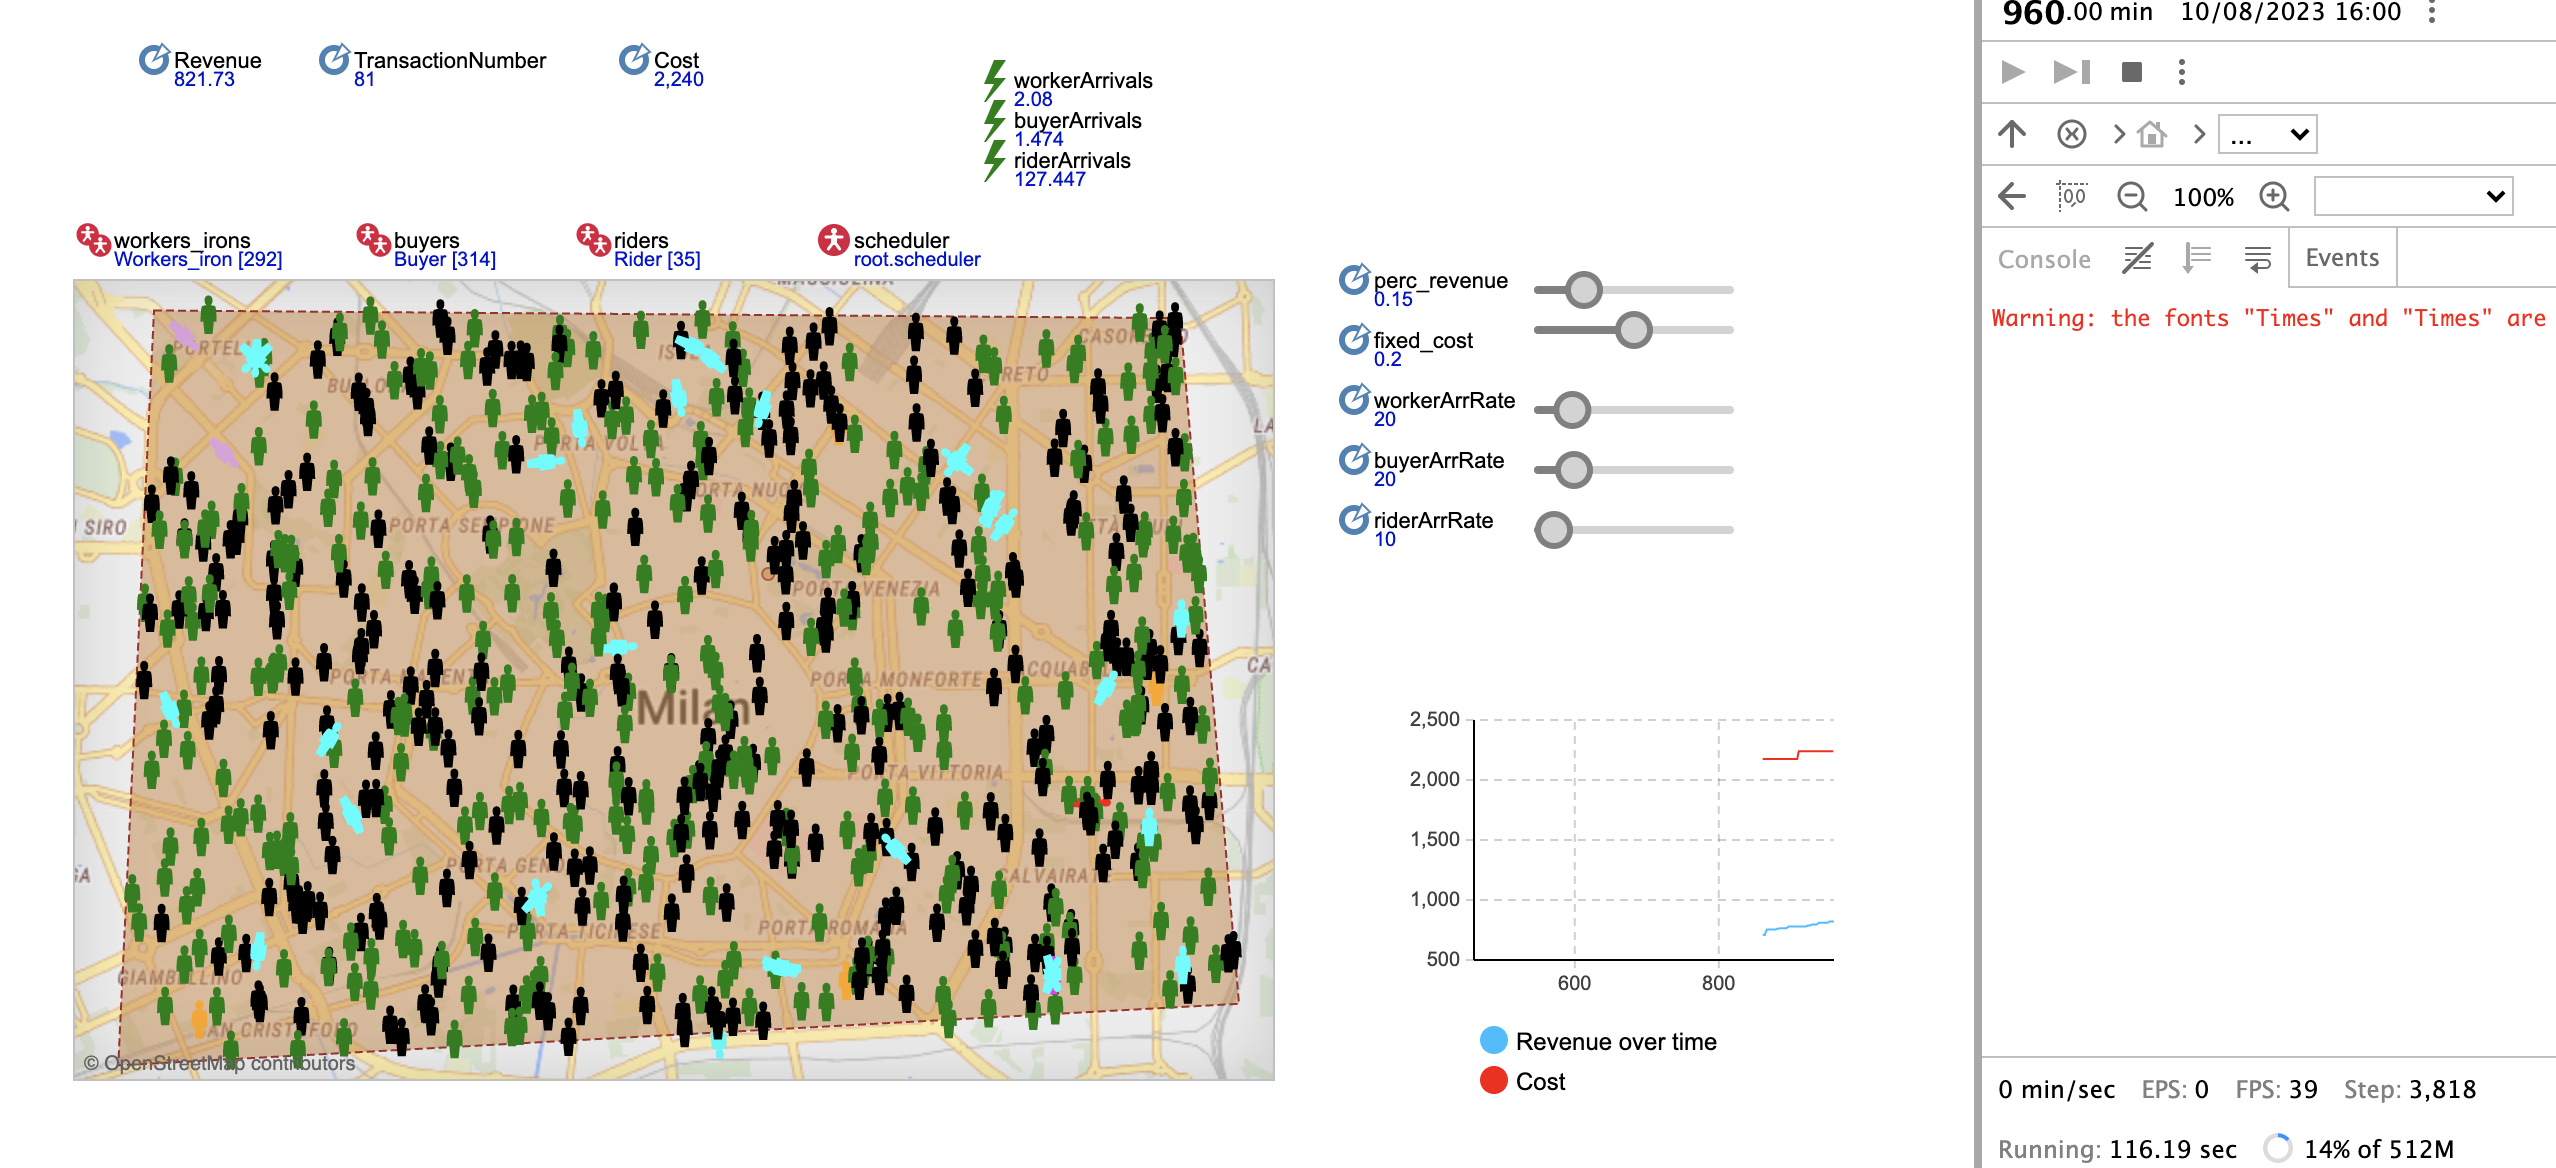
\includegraphics[scale=0.3]{../Images/sim01.png}
\end{figure}
As you can see from the top KPI or form the chart in the bottom-right side the Revenue are below the Cost. So there will be a lost over the first day. So we need to change some parameters and check if the situation will be better or not. For doing that I applied the What-If scenario different time as reported below.
\subsection{What-If scenario 1: }